\documentclass[11pt,twocolumn,oneside,openany,headings=optiontotoc,11pt,numbers=noenddot]{article}

\usepackage[a4paper]{geometry}
\usepackage[utf8]{inputenc}
\usepackage[T1]{fontenc}
\usepackage{lmodern}
\usepackage[ngerman]{babel}
\usepackage{ngerman}

\usepackage[onehalfspacing]{setspace}

\usepackage{fancyhdr}
\usepackage{fancybox}

\usepackage{rotating}
\usepackage{varwidth}

%Struktogramme
\usepackage[german,curves]{struktex}

\usepackage{pdflscape}
\usepackage{changepage}
\usepackage{graphicx}
\usepackage[bottom]{footmisc}
\usepackage{transparent}
\usepackage{graphbox}
\graphicspath{
	{Pics/PDFs/}
	{Pics/JPGs/}
	{Pics/PNGs/}
}
\usepackage{caption}
\usepackage{wrapfig}
\usepackage{marginnote}
\usepackage{tabularx}
\usepackage{dashrule}
\usepackage{soulutf8}
\usepackage{hhline}
%arydshln suppresses vertical lines in table
%\usepackage{arydshln}
\usepackage{multirow}
\usepackage{enumerate}
\usepackage[hidelinks]{hyperref}
\usepackage{listings}

\usepackage[table]{xcolor}
\usepackage{array}
\usepackage{enumitem,amssymb,amsmath}
\usepackage{interval}
\usepackage{cancel}
\usepackage{stmaryrd}
\usepackage{wasysym}
\usepackage{polynom}
\usepackage{diagbox}
\usepackage{dashrule}
\usepackage{framed}
\usepackage{mdframed}
\usepackage{karnaugh-map}
\usepackage{pdfpages}

\usepackage{blindtext}

\usepackage{eso-pic}

\usepackage{amssymb}
\usepackage{eurosym}

\usepackage[pages=some]{background}
\pagestyle{headings}
\renewcommand{\headrulewidth}{0.2pt}
\renewcommand{\footrulewidth}{0.2pt}
\newcommand*{\underdownarrow}[2]{\ensuremath{\underset{\overset{\Big\downarrow}{#2}}{#1}}}
\setlength{\fboxsep}{5pt}
\newcommand{\explainBelow}[3]{\underbrace{#1}_{\parbox{\widthof{#3}}{\footnotesize\raggedright #2}}}
\newcommand{\explainAbove}[3]{\overbrace{#1}^{\parbox{\widthof{#3}}{\footnotesize\raggedright #2}}}
\newcommand\footnoteref[1]{\protected@xdef\@thefnmark{\ref{#1}}\@footnotemark}


% Codestyle defined
\definecolor{codegreen}{rgb}{0,0.6,0}
\definecolor{codegray}{rgb}{0.5,0.5,0.5}
\definecolor{codepurple}{rgb}{0.58,0,0.82}
\definecolor{backcolour}{rgb}{0.95,0.95,0.92}
\definecolor{deepgreen}{rgb}{0,0.5,0}
\definecolor{darkblue}{rgb}{0,0,0.65}
\definecolor{mauve}{rgb}{0.40, 0.19,0.28}
\colorlet{exceptioncolour}{yellow!50!red}
\colorlet{commandcolour}{blue!60!black}
\colorlet{numpycolour}{blue!60!green}
\colorlet{specmethodcolour}{violet}

%Neue Spaltendefinition
\newcolumntype{L}[1]{>{\raggedright\let\newline\\\arraybackslash\hspace{0pt}}m{#1}}
\newcolumntype{M}{>{\centering\arraybackslash}X}
\newcommand{\cmnt}[1]{\ignorespaces}
%Textausrichtung ändern
\newcommand\tabrotate[1]{\rotatebox{90}{\raggedright#1\hspace{\tabcolsep}}}

%Intervall-Konfig
\intervalconfig {
	soft open fences
}

%Bash
\lstdefinestyle{BashInputStyle}{
	language=bash,
	basicstyle=\small\sffamily,
	backgroundcolor=\color{backcolour},
	columns=fullflexible,
	backgroundcolor=\color{backcolour},
	breaklines=true,
}
%Java
\lstdefinestyle{JavaInputStyle}{
	language=Java,
	backgroundcolor=\color{backcolour},
	aboveskip=1mm,
	belowskip=1mm,
	showstringspaces=false,
	columns=flexible,
	basicstyle={\footnotesize\ttfamily},
	numberstyle={\tiny},
	numbers=none,
	keywordstyle=\color{purple},,
	commentstyle=\color{deepgreen},
	stringstyle=\color{blue},
	emph={out},
	emphstyle=\color{darkblue},
	emph={[2]rand},
	emphstyle=[2]\color{specmethodcolour},
	breaklines=true,
	breakatwhitespace=true,
	tabsize=2,
}
%Python
\lstdefinestyle{PythonInputStyle}{
	language=Python,
	alsoletter={1234567890},
	aboveskip=1ex,
	basicstyle=\footnotesize,
	breaklines=true,
	breakatwhitespace= true,
	backgroundcolor=\color{backcolour},
	commentstyle=\color{red},
	otherkeywords={\ , \}, \{, \&,\|},
	emph={and,break,class,continue,def,yield,del,elif,else,%
		except,exec,finally,for,from,global,if,import,in,%
		lambda,not,or,pass,print,raise,return,try,while,assert},
	emphstyle=\color{exceptioncolour},
	emph={[2]True,False,None,min},
	emphstyle=[2]\color{specmethodcolour},
	emph={[3]object,type,isinstance,copy,deepcopy,zip,enumerate,reversed,list,len,dict,tuple,xrange,append,execfile,real,imag,reduce,str,repr},
	emphstyle=[3]\color{commandcolour},
	emph={[4]ode, fsolve, sqrt, exp, sin, cos, arccos, pi,  array, norm, solve, dot, arange, , isscalar, max, sum, flatten, shape, reshape, find, any, all, abs, plot, linspace, legend, quad, polyval,polyfit, hstack, concatenate,vstack,column_stack,empty,zeros,ones,rand,vander,grid,pcolor,eig,eigs,eigvals,svd,qr,tan,det,logspace,roll,mean,cumsum,cumprod,diff,vectorize,lstsq,cla,eye,xlabel,ylabel,squeeze},
	emphstyle=[4]\color{numpycolour},
	emph={[5]__init__,__add__,__mul__,__div__,__sub__,__call__,__getitem__,__setitem__,__eq__,__ne__,__nonzero__,__rmul__,__radd__,__repr__,__str__,__get__,__truediv__,__pow__,__name__,__future__,__all__},
	emphstyle=[5]\color{specmethodcolour},
	emph={[6]assert,range,yield},
	emphstyle=[6]\color{specmethodcolour}\bfseries,
	emph={[7]Exception,NameError,IndexError,SyntaxError,TypeError,ValueError,OverflowError,ZeroDivisionError,KeyboardInterrupt},
	emphstyle=[7]\color{specmethodcolour}\bfseries,
	emph={[8]taster,send,sendMail,capture,check,noMsg,go,move,switch,humTem,ventilate,buzz},
	emphstyle=[8]\color{blue},
	keywordstyle=\color{blue}\bfseries,
	rulecolor=\color{black!40},
	showstringspaces=false,
	stringstyle=\color{deepgreen}
}

\lstset{literate=%
	{Ö}{{\"O}}1
	{Ä}{{\"A}}1
	{Ü}{{\"U}}1
	{ß}{{\ss}}1
	{ü}{{\"u}}1
	{ä}{{\"a}}1
	{ö}{{\"o}}1
}

% Neue Klassenarbeits-Umgebung
\newenvironment{worksheet}[3]
% Begin-Bereich
{
	\newpage
	\sffamily
	\setcounter{page}{1}
	\ClearShipoutPicture
	\AddToShipoutPicture{
		\put(55,761){{
				\mbox{\parbox{385\unitlength}{\tiny \color{codegray}BBS I Mainz, #1 \newline #2
						\newline #3
					}
				}
			}
		}
		\put(455,761){{
				\mbox{\hspace{0.3cm}
\includegraphics[width=0.2\textwidth]{../../logo.pdf}}
			}
		}
	}
}
% End-Bereich
{
	\clearpage
	\ClearShipoutPicture
}

\setlength{\columnsep}{3em}
\setlength{\columnseprule}{0.5pt}

\geometry{left=2.50cm,right=2.50cm,top=3.00cm,bottom=1.00cm,includeheadfoot}
\pagenumbering{arabic}
\pagestyle{plain}

\begin{document}
	\begin{worksheet}{Höhere Berufsfachschule IT-Systeme}{Grundstufe - Mathematik}{Grundlagen Funktionen - Funktionsbegriff, Wertetabelle, Graph}
		\setcounter{section}{7}
		\section{Begriffe zur Beschreibung eines Graphen}
		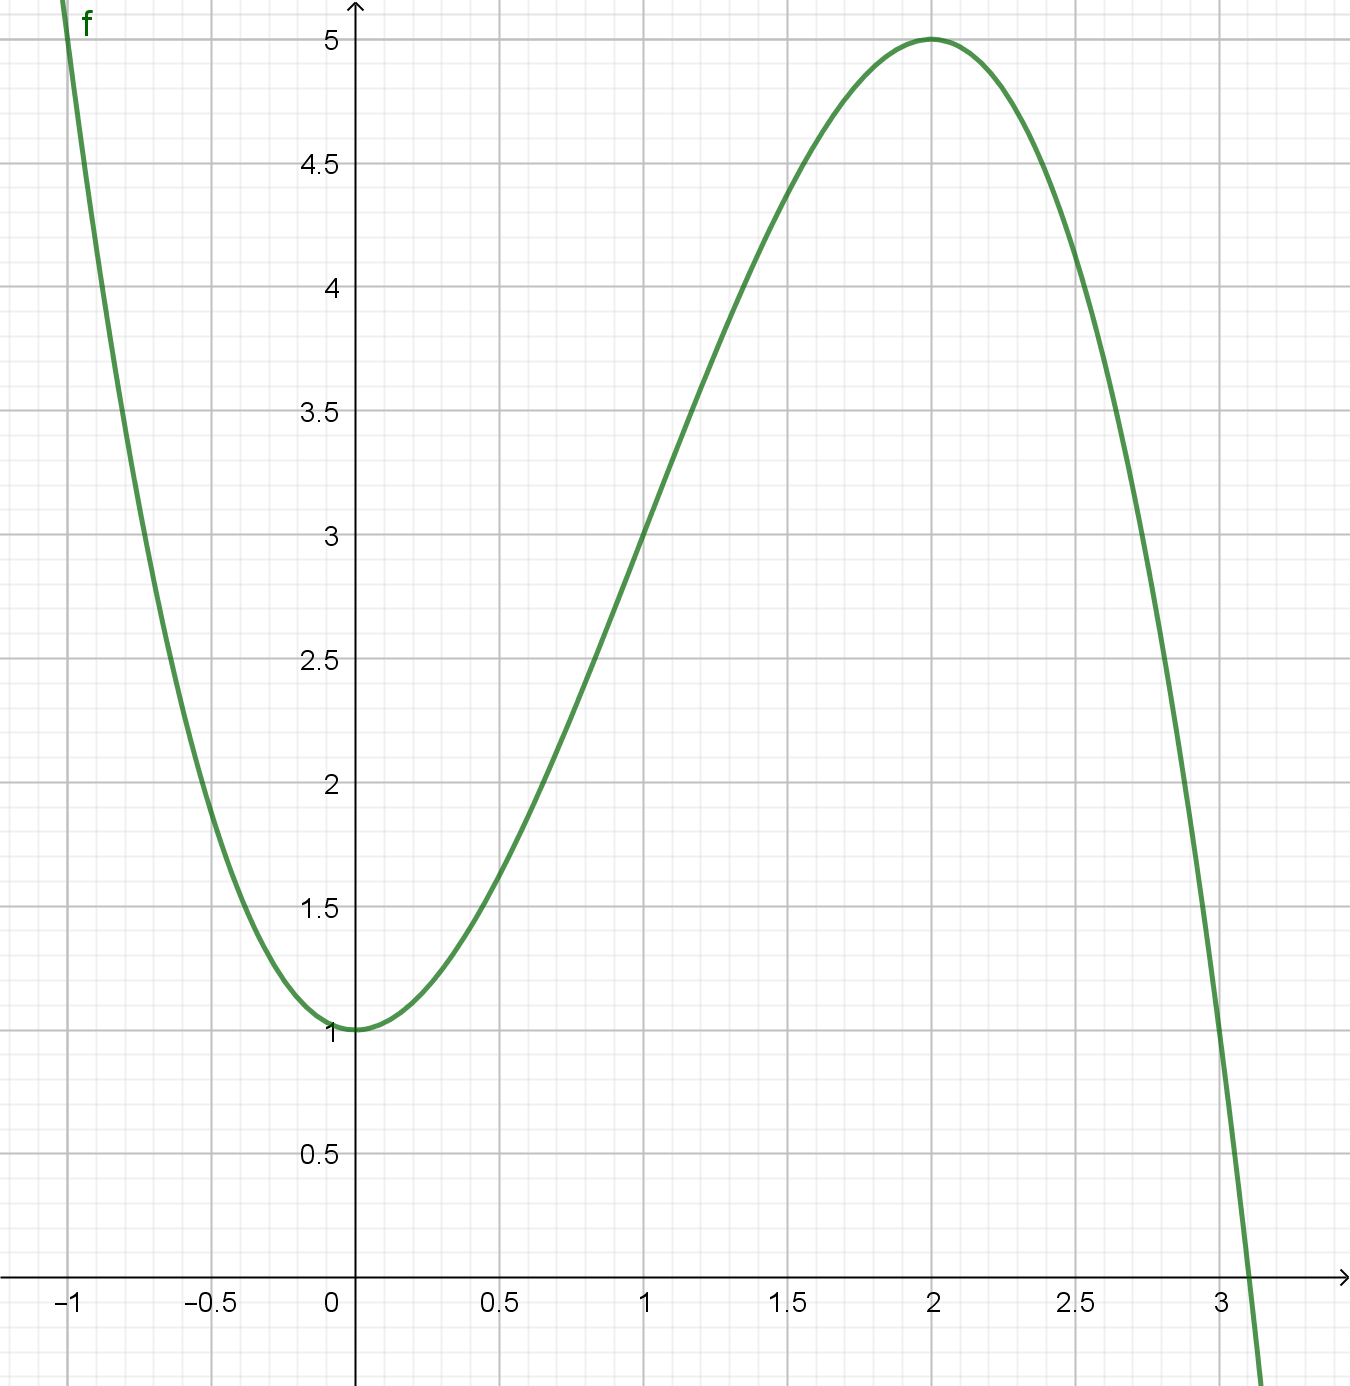
\includegraphics[width=0.49\textwidth]{../99_Bilder/basicsBsp.png}\\
		\par\bigskip\noindent
		Stellen Sie sich vor, Sie müssten den oben dargestellten Graphen am Telefon beschreiben. Welche Charakteristika würden Sie nennen?
		\subsection*{y-Achsenabschnittswert}
		Der Wert, bei dem der Graph die y-Achse schneidet, nennt man \textbf{\underline{y-Achsenabschnitt}}. Rechnerisch erhält man diesen Wert dadurch, dass man \(x= 0\) besetzt.\\
		\par\bigskip\noindent
		\textbf{Wichtig: Die y-Achse hat \underline{Werte}.}
		\subsection*{Nullstelle(n)}
		Die Stellen, an denen der Graph die x-Achse schneidet, nennt man \textbf{\underline{Nullstellen}}. Um diese Nullstellen zu berechnen, löst man die Gleichung \(y = 0\).\\
		\par\bigskip\noindent
		\textbf{Achtung: Auf der x-Achse gibt es nur \underline{Stellen}.}\\
		\includegraphics[width=0.49\textwidth]{../99_Bilder/nyAA.png}\\
		\par\bigskip\noindent
		Existieren mehrere Nullstellen, so markiert man dies durch Indizies an der Variable x (\(x_1, x_2, x_3, \ldots\))
		\subsection*{Monoton steigend/fallend}
		Werden die \underline{y-Werte mit zunehmendem x} über einem Intervall immer \underline{größer}, so nennt man den dazugehörigen Graphen \textbf{\underline{monoton steigend}} über dem entsprechenden Intervall.\\
		Werden die \underline{y-Werte mit zunehmendem x} hingegen immer \underline{kleiner}, so spricht man von einem \textbf{\underline{monoton fallenden}} Graphen über dem Intervall.\\
		Die entsprechenden Intervalle gibt man dann so an:\\
		Monoton fallend \(\left[-\infty;0\right]\)\\
		Monoton fallend \(\left[0;2\right]\)\\
		Monoton fallend \(\left[2;\infty\right]\)
		\subsection*{Extremstelle}
		Findet ein Wechsel von monoton fallend zu monoton steigend bzw. von monoton steigend zu monoton fallend statt, haben wir an dieser Stelle eine \underline{\textbf{Extremstelle}}.\\
		Der dazugehörige \underline{y-Wert} wird auch \underline{\textbf{relatives Minimum/relatives Maximum}} genannt. Dabei handelt es sich um den niedrigsten/höchsten Funktionswert in einer bestimmten Umgebung um diese Extremstelle.\\
		Den dazugehörigen Punkt nennt man \textbf{\underline{Tief- bzw. Hochpunkt}}.\\
		\textit{Sprechweise: Beachten Sie, dass ein Graph immer \underline{über} einem Intervall steigt oder fällt - unabhängig davon, ob der Graph oberhalb oder unterhalb der x-Achse verläuft.}\\
		\par\bigskip\noindent
		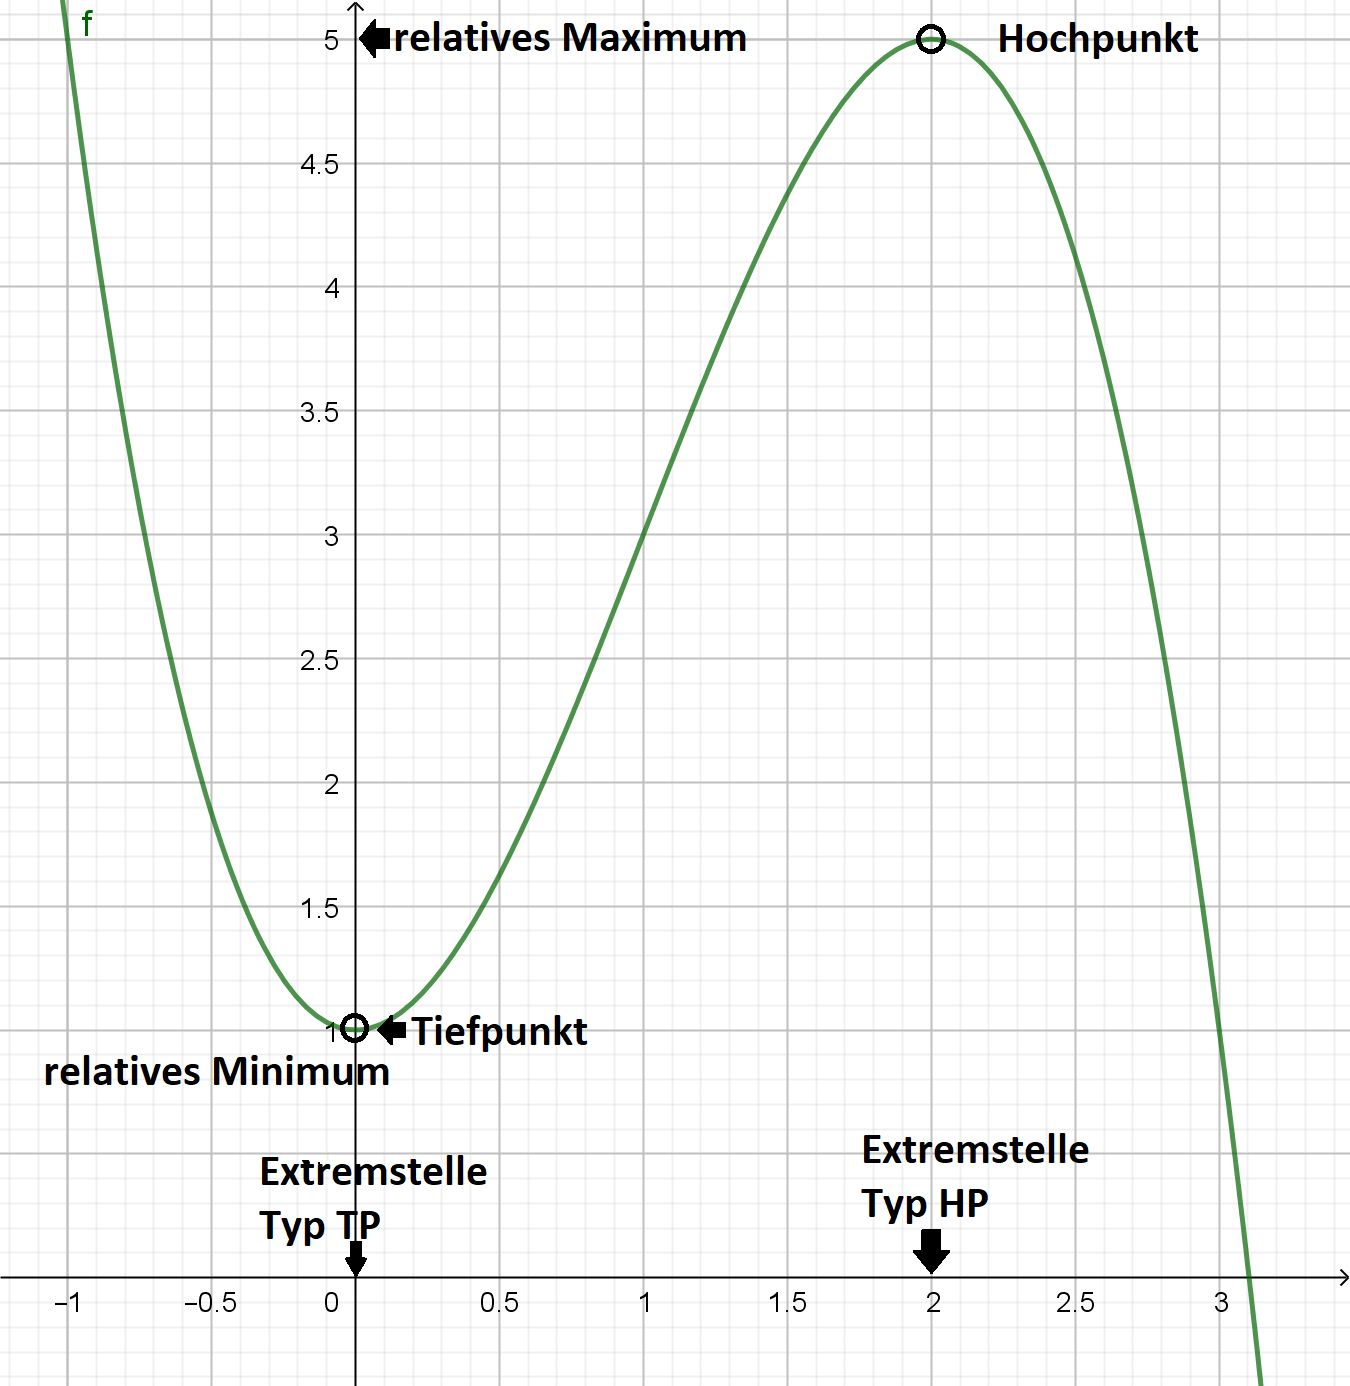
\includegraphics[width=0.49\textwidth]{../99_Bilder/EP.png}\\
		\par\bigskip\noindent
		Der Graph hat Extremstellen bei \(x_{TP} = 0\) und \(x_{HP} = 2\).\\
		Die dazugehörigen Punkte \textbf{Tiefpunkt (0|1)} und \textbf{Hochpunkt (2|5)}.\\
		Daraus können die relativen Minima bzw. Maxima ablesbar. So ergibt sich das \textbf{relative Minimum} bei \( y_{MIN} = 1\) und das \textbf{relative Maximum} bei \(y_{MAX} = 5\).
		\subsection*{Krümmungsverhalten und Wendestelle}
		Stellt man sich den Graphen als einen Berg vor, ist logisch, dass es ab der Extremstelle \(x_{TP} = 0\) aufwärts geht, man also ansteigt. Zunächst wird die Steigung immer größer, also steiler. Ab der Stelle \(x = 1\) steigt man zwar weiterhin an, aber die Intensität der Steigung wird weniger - also flacht der Berg langsam ab.\\
		Diesen Wechsel kann man mit dem \textbf{Krümmungsverhalten} beschreiben. Die Stelle, an der sich das Krümmungsverhalten änder, nennt man \textbf{\underline{Wendestelle}}. Der dazugehörige Punkt heißt \underline{Wendepunkt}.\\
		\par\bigskip\noindent
		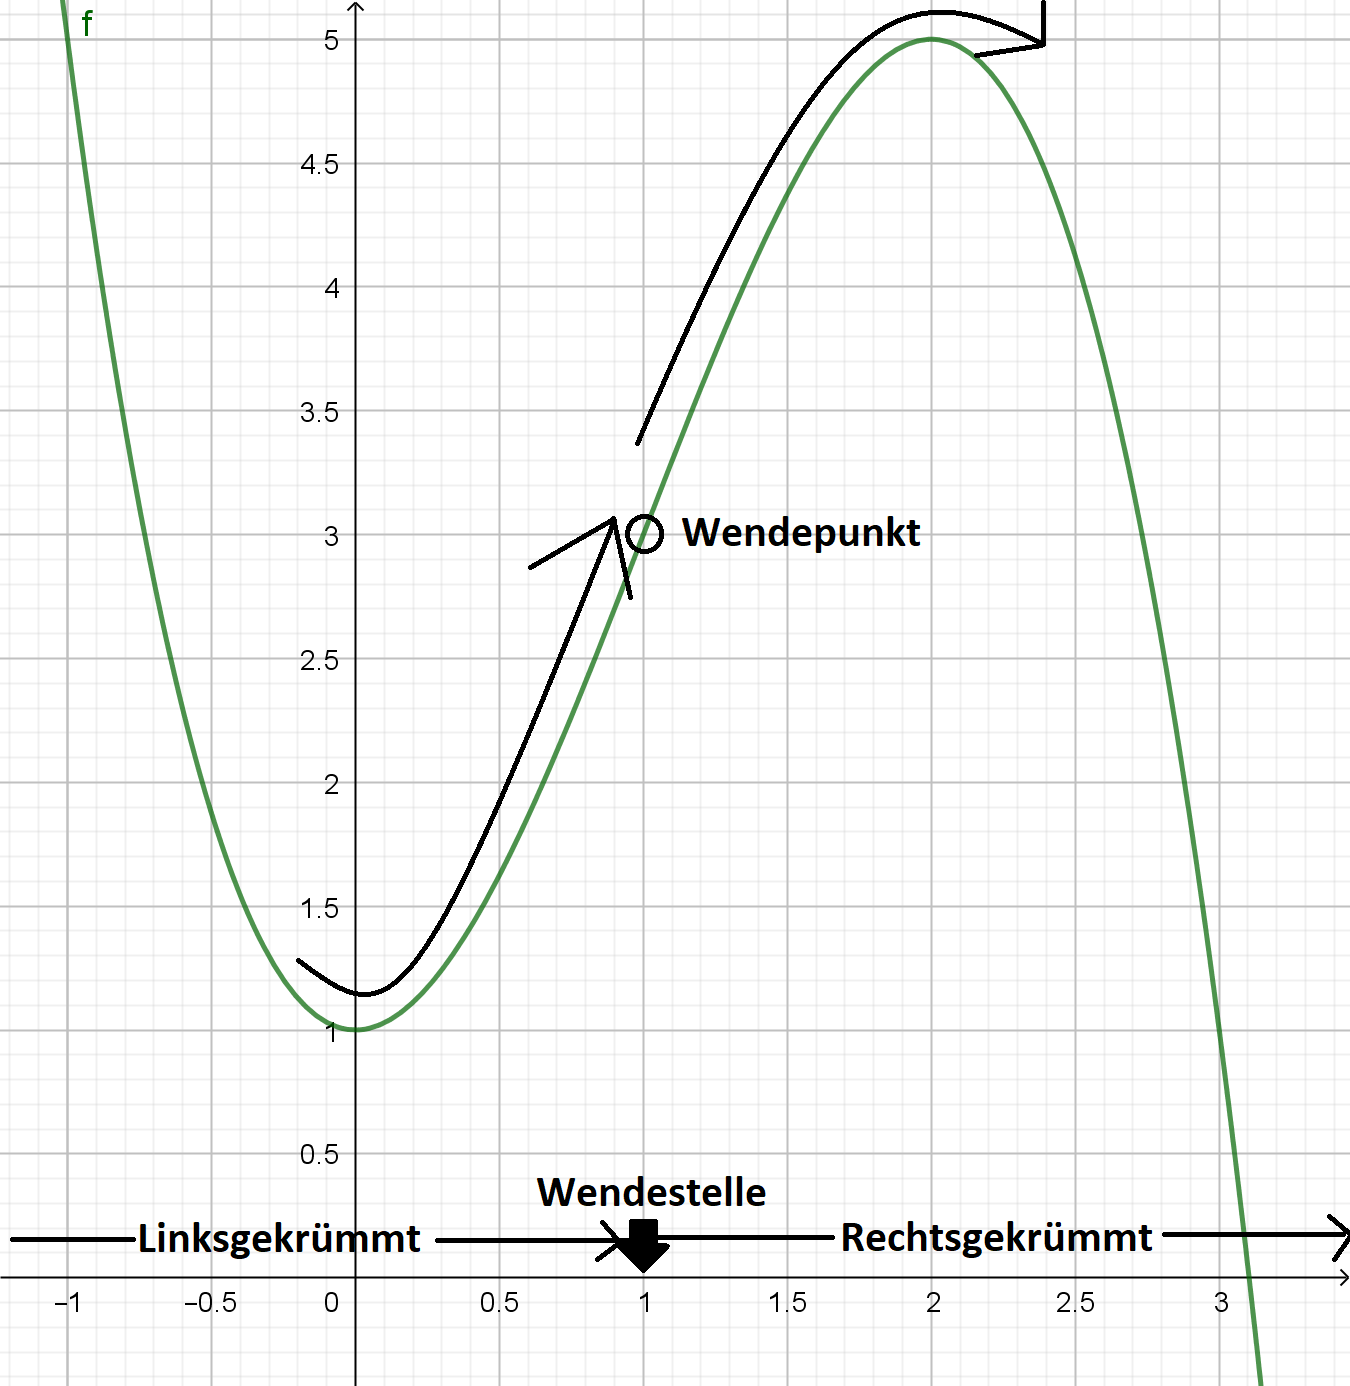
\includegraphics[width=0.49\textwidth]{../99_Bilder/WP.png}\\
		\par\bigskip\noindent
		\textit{Wichtig ist, dass das Krümmungsverhalten wie angegeben, \glqq{}links-\grqq{} bzw. \glqq{}rechtsgekrümmt\grqq{} nur korrekt ist, wenn man den Graph mit dem Auge entsprechend der Orientierung der x-Achse, also on positive x-Richtung, verfolgt.\\ Daher ist das Anbringen eines weiteren Pfeils links an der x-Achse strengstens untersagt.}
	\end{worksheet}
\end{document}